\chapter{Properties of LSCO}

\begin{framed}
    \begin{itemize}
        \item \textbf{Find a better title}
        \item Dopants (LSCO, LCO+O, LSCO+O, LNSCO, LBCO)
        \item Phase diagram (Tc, Tn, T* - macro stuff). How things are measured. Specific heat, Magnetization etc.
        \item Stripe order (why do we think it is important?). 
        \item Phase diagram including microscopic measurements (such as Kofu's).
        \item Other microscopic measured phenomena (I can only think of loop currents, others?)
        \item Theories (PDW, RVB, Loop currents, spin-fluctuation mediated SC). Are these even the same level of theory?
        \item Structural aspects of LSCO (The LTT problem, LBCO, LNSCO, define Q1 Q2, Superstripes). This should feed right into the motivation of the thesis.
        \item The relationship between ordering (such as stripes) and electronic band structure (from ARPES etc).
    \end{itemize}
\end{framed}

In this chapter, we look more closely at a specific family cuprates derived from La$_2$CuO$_4$, relevant to this thesis. Since one has to be careful about extrapolating conclusions based on specific samples to unconventional superconductivity as a whole, I will attempt to provide the broader context when applicable. While this chapter will primarily survey experiments and theories relevant to the work performed in this thesis, I emphasize the almost unmanageable amount of novel phenomena discovered in these compounds. It is my strong belief that `solving' the cuprates will require clues from many areas of research and it is my intention to highlight some of these clues here, even when outside the scope of this thesis.

\begin{figure}
    \centering
    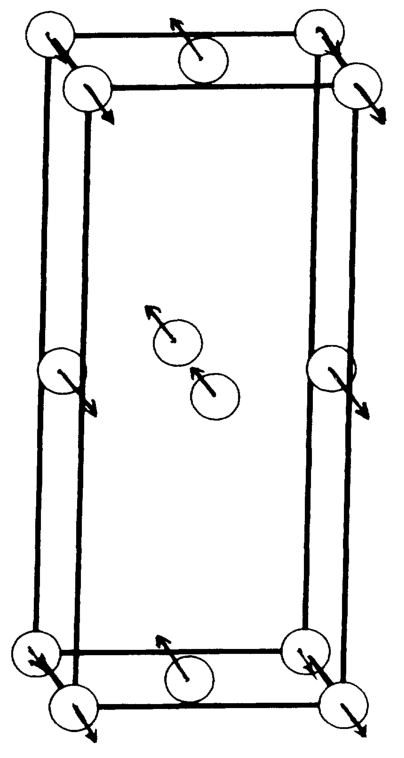
\includegraphics[width=0.5\textwidth]{fig/lsco/lsco_afm.png}
    \caption[AFM structure of LSCO]{AFM structure of LSCO}
    \label{fig:lsco_afm}
\end{figure}